\chapter{Implementation}
This chapter will explain how the described concept has been implemented.
First an overview of the concept and then the main parts of the software in more
detail.
The trackable marker is attached to the ultrasound probe. The marker is
detectable by the tracking camera and enables the camera to determine the
position and orientation of the ultrasound probe. The probe on its own will
create an ultrasound image. Then the sampled ultrasound image and pose will be
post processed as a pair in the computer. In the software, depending on the
actual state of the surgery, the use of the two will be different.

\begin{figure}[H]
  \centering
 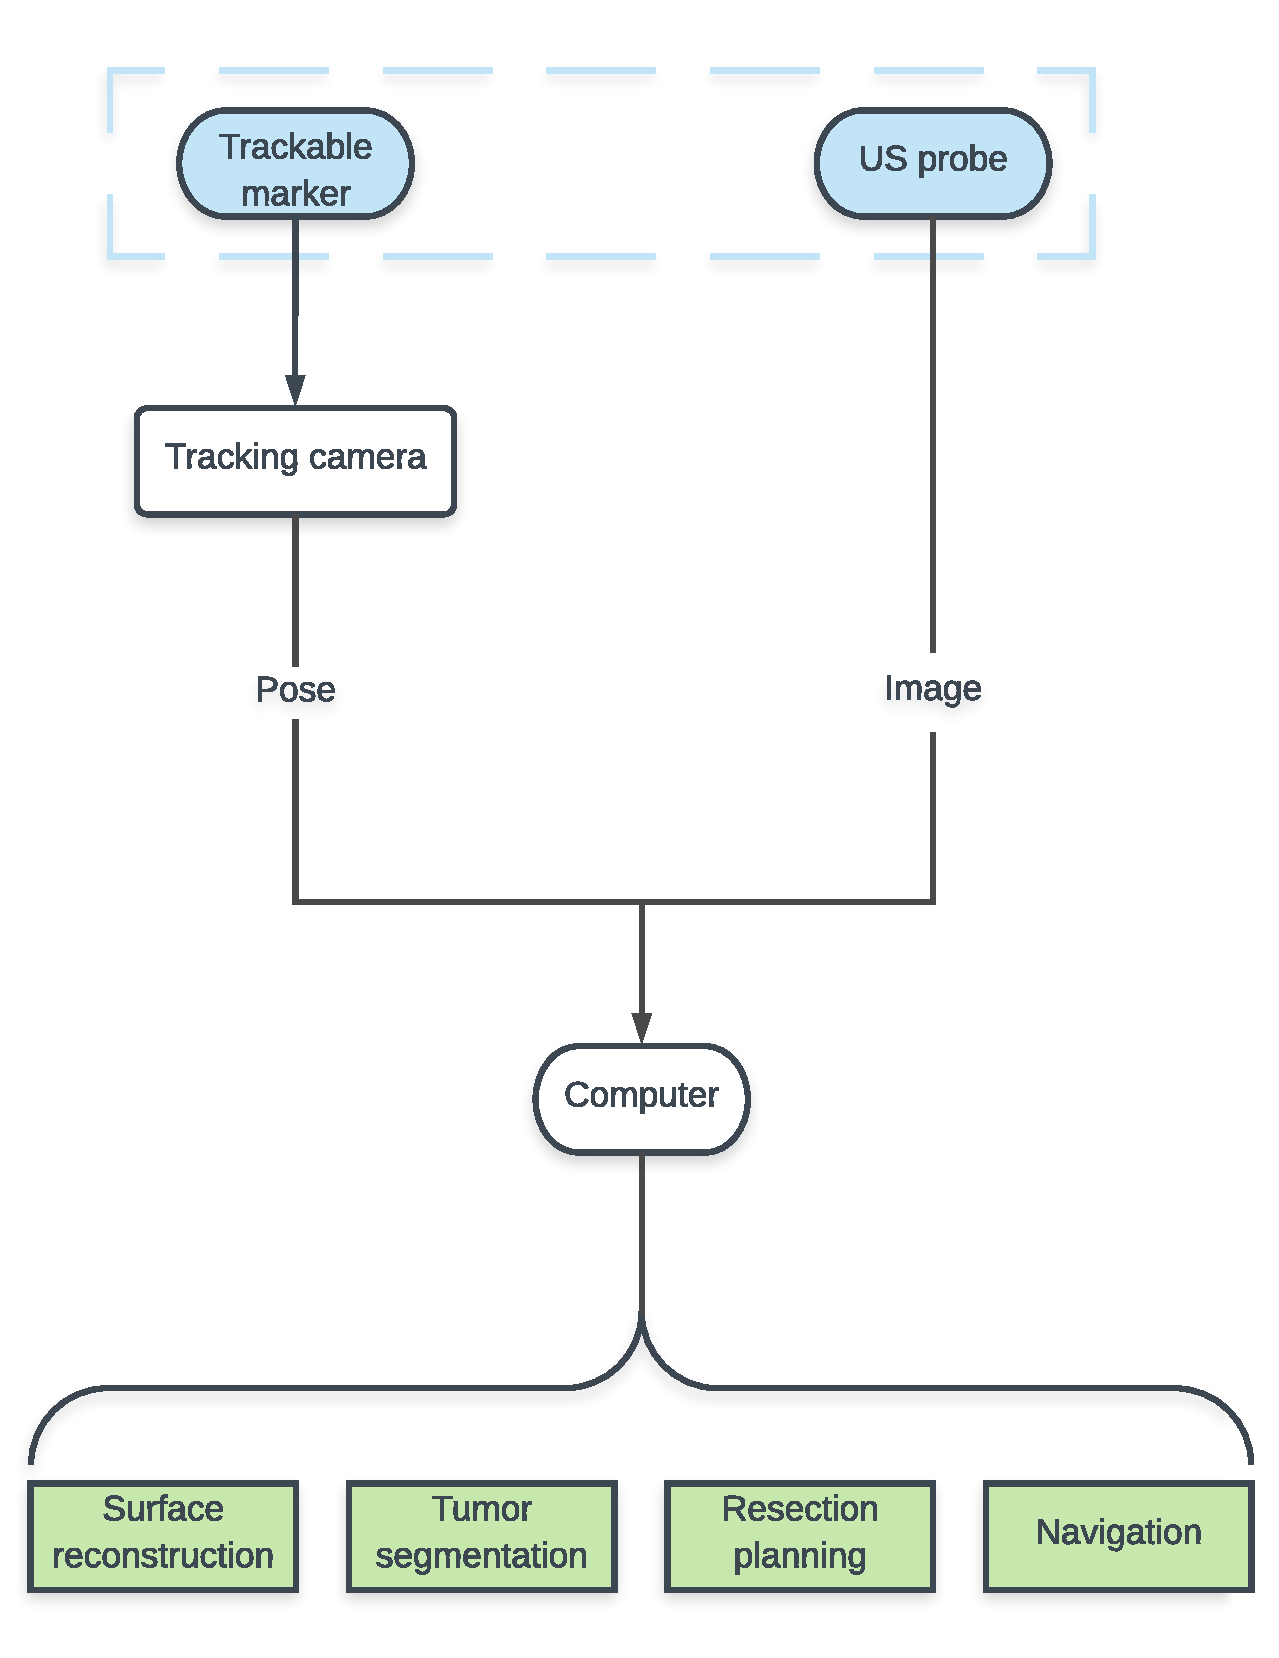
\includegraphics[width=0.6\textwidth]{FirstFlowChart}
  \caption{The way of the ultrasound image and the corresponding pose to the
    computer and later to the different parts in the software.}
  \label{fig:FirstFlowChart}
\end{figure}

\section{Surface Reconstruction}
While the surgeon is scanning the surface, the software in the background
filters out unusable positions. An image pose pair has to take two hurdles to
become accepted in the group of surface points. The image has to prove that it
arised from the liver surface and the position has to have a similar distance to
its neighbors as its neighbors to it. 
When enough points are sampled, the reconstruction of the surface will be
carried out.
\begin{figure}[H]
  \centering
 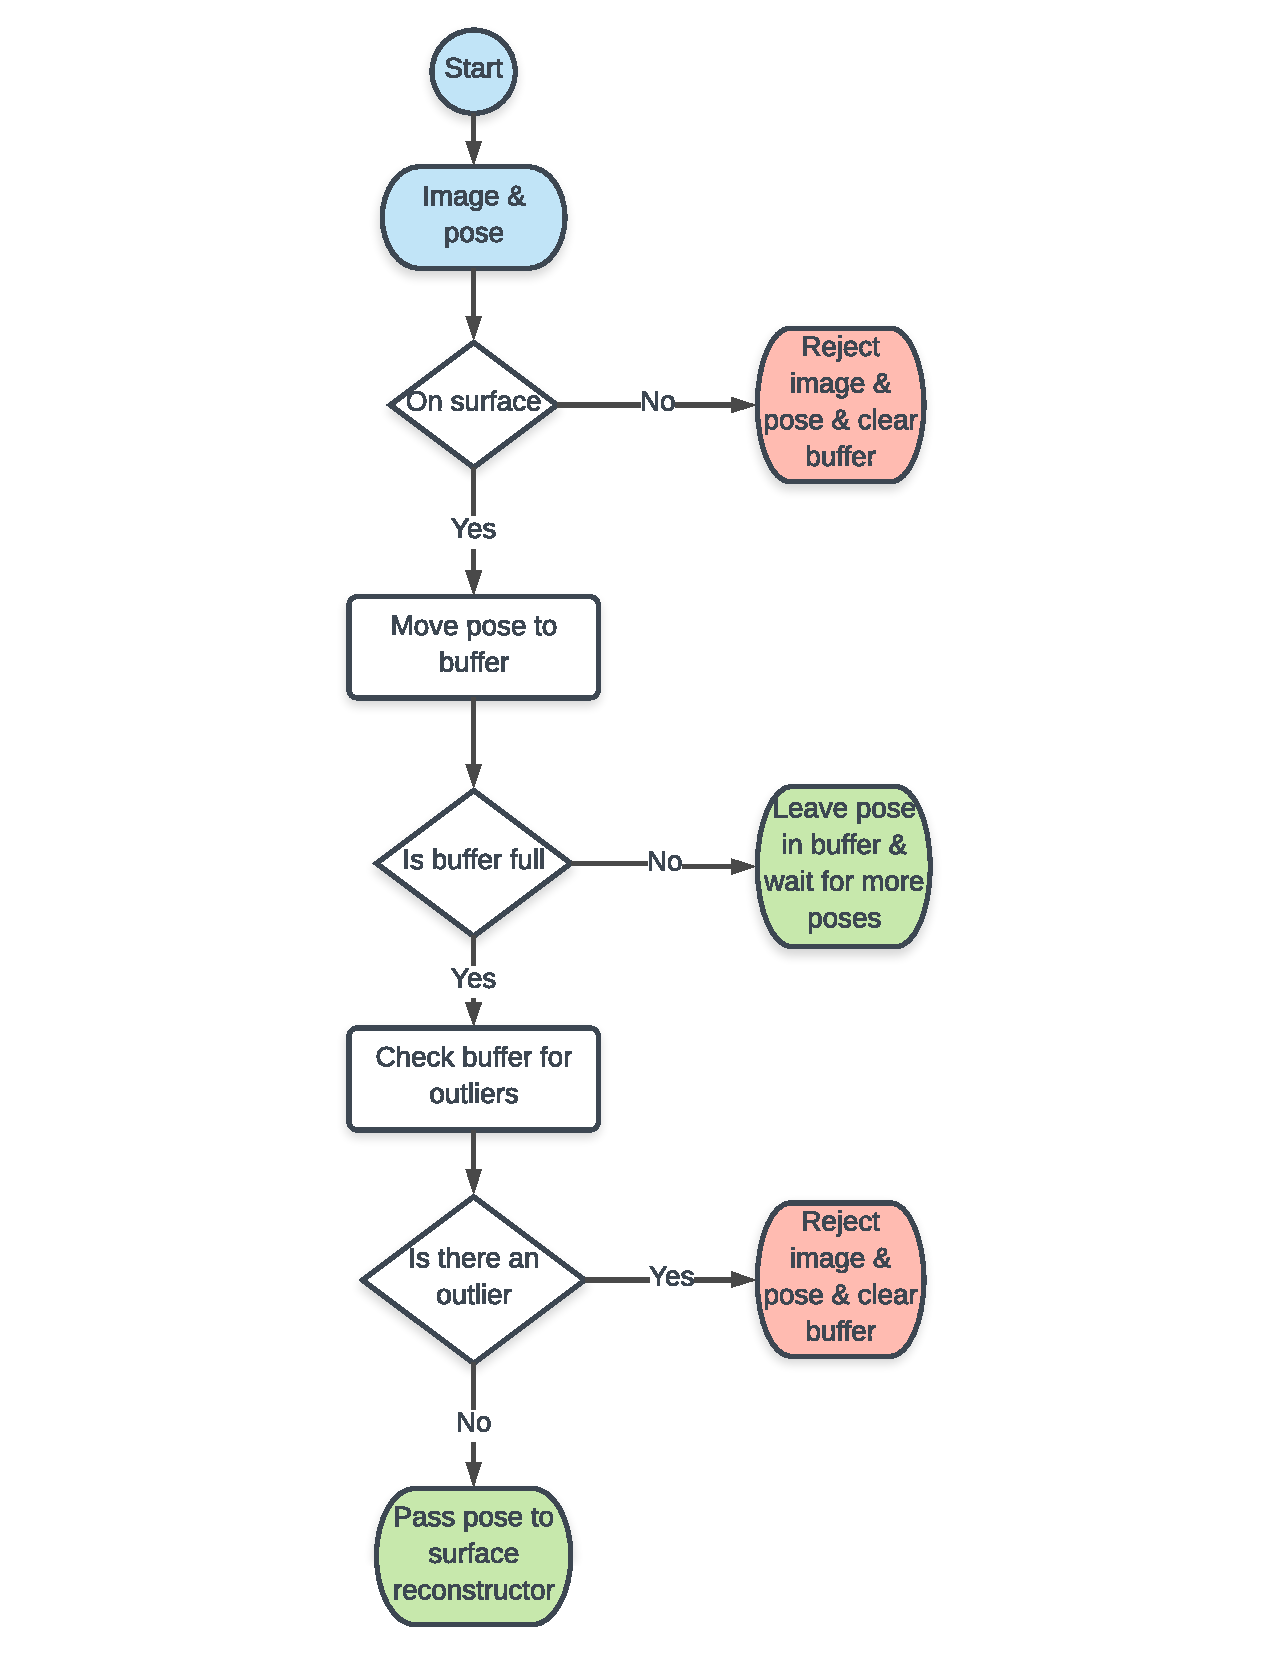
\includegraphics[width=0.6\textwidth]{SecondFlowChart}
  \caption{The way of the image and its pose if the surgeon is scanning the
    surface.}
  \label{fig:SecondFlowChart}
\end{figure}

\subsection{Surface contact detection}
For an image pose pair, the first step to pass is the contatct detection. Only
the ultrasound image is needed in this step. 

\begin{figure}[H]
  \centering
  \minipage{0.32\linewidth}
  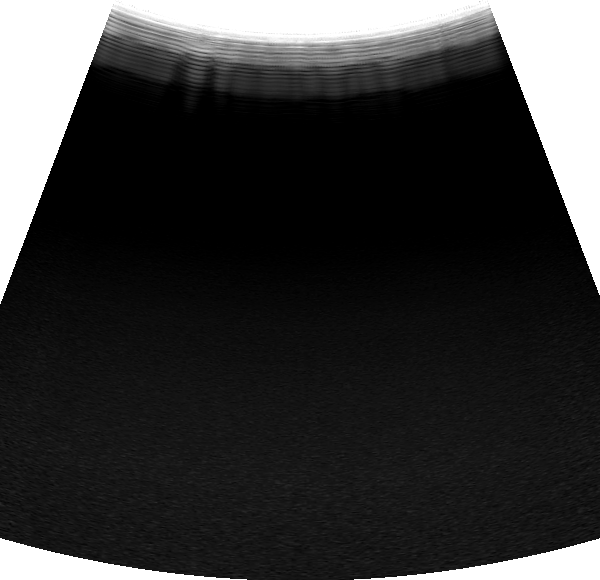
\includegraphics[width=\linewidth]{contact_no}
  \endminipage
  \hfill
  \minipage{0.32\linewidth}
  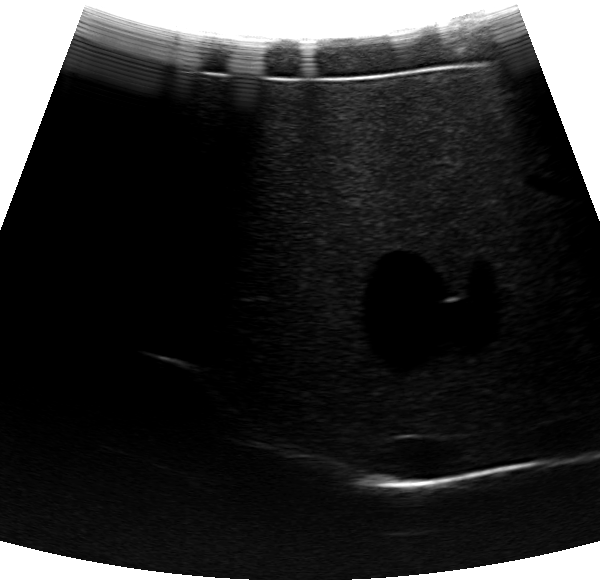
\includegraphics[width=\linewidth]{contact_difficult}
  \endminipage
  \hfill
  \minipage{0.32\linewidth}
  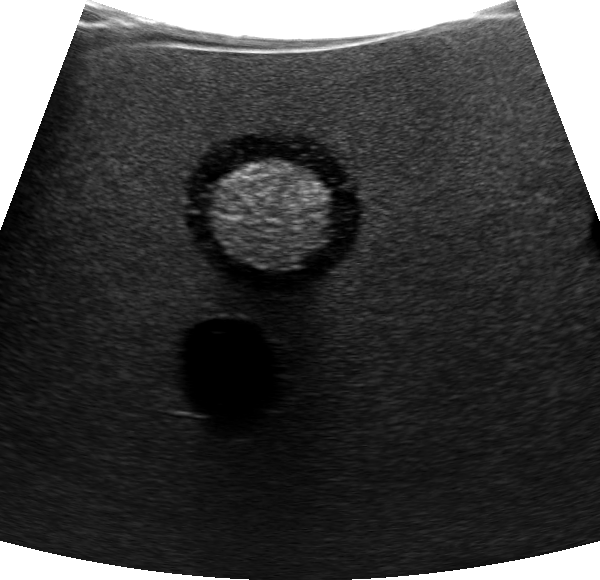
\includegraphics[width=\linewidth]{contact}
  \endminipage
  \hfill 
 \caption{Three ultrasound images from left to right: No contact with the liver,
   difficult to decide (In this case it would be contact because the middle part
   of the image shows contact), contact with the liver}
  \label{fig:contactVSnocontact}
\end{figure}

A classifier detects whether the US probe has contact to the liver or not. Therefore, a support vector machine (SVM) was trained with US images
from the phantom and from previous navigated liver surgeries. The SVM was trained to
classify the image into ``no surface contact'' (left) and ``surface contact'' (middle and right).
The images were labelled as "surface contact" if at least 50\% and the center had contact
to the surface (Figure 6.4 middle). The classifier takes into account that US waves are
reflected at the US probe-air interface when the US probe has no contact to the liver and
therefore no image is formed. The features for the classifier were: mean, median, minimum,
maximum, variance, skewness and kurtosis of the pixel values. All features are calculated
on the upper half of the image. For training, a set of 2'311 images (1'056 with contact, 1'255
without contact) were used. The training data was composed of images from a phantom
(88\%) and images from previous navigated liver surgeries (12\%). All computations were
performed using the SciPy software package.
\subsection{Outlier removal}
When the image is classified as ``surface contact'', then the position of the pose is shuffled
into the buffer. The buffer has a capacity for 10 positions. When
the addition of the actual pose leads to a full buffer, the buffer is
tested for outliers. To find outliers in the current buffer the local
outlier factor is calculated for each position. 

\subsubsection{Local outlier factor (LOF)}
The local outlier factor is a numerical value that describes the local density
of a position depending on and compared to its k-nearest neighbors. BBLBLBLBL
steps can be separeted to find the LOF of one position.
\begin{enumerate}
  \item{For each point calculate the distance to all the other points in the buffer}
  \item{For each point find the distance to his k-nearest neighbor $\rightarrow$
    this is called the \textit{k-distance} for this point}
  \item{Find the \textit{reachability distance} from the k-nearest neighbors
      of each point to it self}
  % \item{Find the \textit{ reachability distances} from the k-nearest neighbors of the
  %     active position to the active position}
  \item{Calculate the \textit{local reachability density} for all points}
  \item{Calculate the \textit{local outlier factor}}
\end{enumerate}

sdfasdfajskldöfjaskdlfaölskdfj aslkdfj asdlkfja The \textit{reachability distance} of point $A$ from another point $B$ is defined:

\begin{gather*}
  \mbox{reachability-distance}_k(A,B)=\max\{\mbox{k-distance}(B), d(A,B)\}
\end{gather*}

\subsection{Reconstruction Parameters}
grid search
\section{Tumor Segmentation}
graph cuts
initialization method
\section{Resection Planning}
\subsection{Cone fitting around tumor}
\section{Visualization for navigation}
\subsection{Ultrasound overlay}
\subsection{3D model}
\section{UI Concept}
%%% Local Variables:
%%% TeX-master: "MscThesis"
%%% End: